\documentclass[a4,12pt]{scrartcl}

%Basic 
\usepackage[utf8]{inputenc}
\usepackage[ngerman]{babel}
\usepackage[T1]{fontenc}
%Schrift 
%\usepackage{fontspec} 
%\setmainfont{Arial} 
%Zeilenabstand
\usepackage{setspace}
\setstretch {1.3}
\usepackage{float}
\usepackage[bottom = 3.50cm]{geometry}

%Titel Seite
\usepackage{titling} %Wird benötigt damit \maketitle die Variabeln title, author und date nicht überschreibt
\title{Test Cases}
%\subtitle{Projekt: software name}
\author{David Meister \and Andreas Stalder}		
 %mit /and können Personen hinzugefügt werden
\date{\today}


%Kopf, Fusszeile
\usepackage{fancyhdr}
\pagestyle{fancy}
\lhead{}
\chead{}
\rhead{Requirements}
\lfoot{\thetitle \: v1.0 }
\cfoot{\today}
\rfoot{Seite \thepage}
\renewcommand{\headrulewidth}{0.4pt}

%Bilder
\usepackage{graphicx}

%Zeichnen
\usepackage{tikz}

%Tabellen
\usepackage{booktabs}
\usepackage{longtable}

%Codesnippets
\usepackage{listings}
\lstset{language=java,basicstyle=\footnotesize,frame=single} %backgroundcolor=\color{lightgray}

%Querformat für eine Seite
\usepackage{lscape}
\usepackage{rotating}
\usepackage{pdflscape}

%URL 
\usepackage[colorlinks=true, linkcolor=blue, urlcolor=blue, citecolor=blue]{hyperref}
\urlstyle{same} 


%Loremimpsum
\usepackage{lipsum}



\begin{document}

%\clearpage\maketitle
\begin{titlepage}
	\centering
	\vspace{5cm}
	\begin{center}
%	\includegraphics[width=0.50\textwidth]{}
	\end{center}
%	{\huge\bfseries software name\par}
	\vspace{8cm}
	\raggedright
	{\bfseries HSR Studienarbeit Network Unit Testing\par}
	{\huge\bfseries Requirements\par}
	\vspace{1cm}
	{\theauthor \par}
	{\today\par}

\end{titlepage}

\section{Änderungsgeschichte}

\begin{table}[htb]
\centering
    \begin{tabular}{@{} l l l l@{}}\toprule    
    {Datum} & {Version} & {Änderung} & {Autor}\\ \midrule
    10.10.16 & 1.0 & Erstellung erster Version & dm/as\\ \addlinespace
    \end{tabular}
\caption{\textbf{Änderungsgeschichte}}
\end{table}

\newpage

%\thispagestyle{empty}
\tableofcontents
\newpage


\section{Einführung}
\subsection{Zweck}
Dieses Dokument beschreibt die Anforderungen mittels Use Cases und nichtfunktionalen
Anforderungen.
\subsection{Gültigkeitsbereich}
Dieses Dokument ist über die gesamte Projektdauer gültig. Es wird in späteren Iterationen angepasst. Somit ist jeweils die neuste Version des Dokuments gültig und alte Versionen sind obsolet.
\subsection{Referenzen}
\begin{itemize}
\item doc/01/Network\_Testing\_Analyse.pdf
\item doc/01/Network\_Testing\_Detailed.pdf

\end{itemize}

\newpage
\section{Allgemeine Beschreibung}
\subsection{Produktperspektive}
Mit Network Unit Tests wird ein automatisches und wiederholbares Testing Framework für Netzwerkumgebungen bereitgestellt. Das Testing der Funktionalitäten im Netzwerk wird meist manuell ausgeführt. Oft werden wichtige Tests vergessen und dadurch Fehler produziert. Mittels automatischem Testen soll ein Werkzeug bereitgestellt werden, um diese Problematik einzudämmen.
\subsection{Produkfunktionen}
Das Programm soll den Anwendern erlauben, Testszenarien zu konfigurieren, auszuführen und auszuwerten. Diese Testszenarien sollen wiederholbar sein, damit sie nach wichtigen Änderungen im Netz einfach ausgeführt werden können.
\subsection{Benutzer Charakteristik}
Zielpersonen sind Netzwerk Engineers, System Administratoren und weitere Informatiker mit Tätigkeit im Netzwerkbereich. Es werden solide Grundkenntnisse in IP-Netzwerken sowie Kenntnisse der verwendeten Netzwerk Devices vorausgesetzt. Der Anwender muss das zu testende Netzwerk im Detail kennen. 
\subsection{Einschränkungen}
Die Software wird auf Linux Plattformen unterstützt. Vorerst werden nur Cisco Netzwerkdevices und Linux Server als zu testende Devices unterstützt.
\newpage
\section{Use Cases}
\subsection{Use Cases Diagramm}
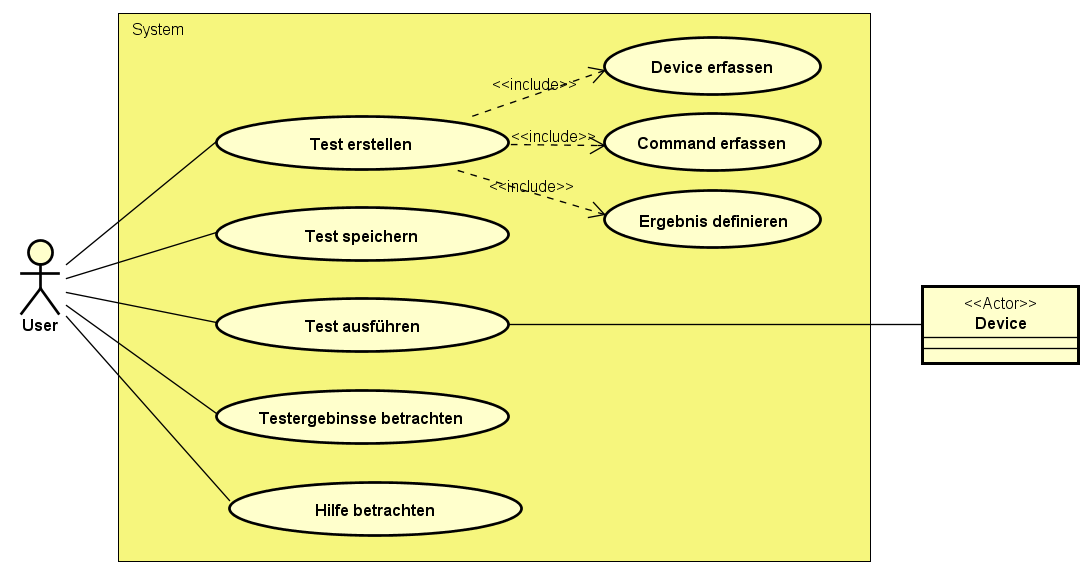
\includegraphics[scale=0.52]{figures/UseCase_Diagram}
\subsection{Aktoren}
Der Benutzer der Applikation ist in diesem System der einzige primäre Aktor. Zu testende Netzwerkdevices agieren als technische Aktoren in diesem System.
\subsection{Beschreibungen (Brief)}
\subsubsection{Test erstellen}
Der User möchte einzelne oder mehrere Tests erstellen. Damit dies möglich ist, sind drei weitere Use Cases nötig.
\paragraph{Device erfassen}\hfill

\noindent Für einen Test sind ein- oder mehrere Devices notwendig. Devices haben Eigenschaften wie Beispielsweise Name, IP-Adresse, Device-Typ (Router, Switch,...) und Login Daten. Diese Devices müssen mittels einem Setup definiert werden.
\paragraph{Command erfassen}\hfill

\noindent Sobald man ein Device erfasst hat, möchte man Kommandos auf diesem ausführen. Dies könnten beispielsweise show-Befehle oder andere Programme zum Senden von Daten sein. Diese Kommandos sind als Queries auf die Devices zu verstehen.

\paragraph{Ergebnis definieren}\hfill

\noindent Sobald Devices und Commands erfasst wurden, kann nun das assert-Statement formuliert werden. Dafür muss das gewünschte Ergebnis definiert werden.

\subsubsection{Test speichern}
Der User hat die Möglichkeit erstellte Tests abzuspeichern um sie später wiederzuverwenden.

\subsubsection{Test ausführen}
Ein fertig formulierter Test kann ausgeführt werden. Mit diesem Vorgang wird die Verbindung zum Device aufgebaut und das im Test definierte Kommando ausgeführt. 

\subsubsection{Testergebnisse betrachten}
Ein ausgeführter Test ist entweder erfolgreich oder er schlägt fehl. Nach ausgeführten Tests kann der User die Testergebnisse betrachten.

\subsubsection{Hilfe betrachten}
Wenn der Benutzer Hilfestellungen benötigt, so kann er die Hilfe betrachten. Die Hilfe bietet Unterstützung für die unterschiedlichen Use Cases.

\newpage
\section{Nichtfunktionale Anforderungen}
In diesem Kapitel behandeln wir die nichtfunktionalen Anforderungen an das Projekt. Wir behandeln Aspekte und Anforderungen aus den Bereichen Qualität, Schnittstellen und Randbedingungen.
\subsection{Qualität}
Bei der Softwarequalität stützen wir uns auf die ISO/IEC 9126 Norm. Es werden die Merkmale Funktionalität, Zuverlässigkeit, Benutzbarkeit, Effizienz, Wartbarkeit und Übertragbarkeit aufgeführt.
\subsubsection{Funktionalität}
Netzwerkdevices können von vielen unterschiedlichen Herstellern kommen. Diese Hersteller verwenden unterschiedliche Syntax und Ausgabeformate. Um die Funktionalität best möglich sicherzustellen, wird die Herstellerunterstützung vorerst stark eingeschränkt. Vorgesehen sind vorerst Cisco Netzwerkdevices und Linux Hosts.
\subsubsection{Zuverlässigkeit}
Tests sind wichtig und nützlich, jedoch nicht Business kritisch bei einem möglichen Ausfall. Es muss vor allem darauf geachtet werden, dass bei ssh Verbindungen ein sauberes Exception Handling implementiert wird, falls beim Verbindungsaufbau oder bei abgesetzten Kommandos etwas schief geht. Es müssen für gewisse Tests auch Timeouts eingeplant werden, damit das Programm nicht unendlich lange blockieren kann.
\subsubsection{Benutzbarkeit}
Wir möchten ein schmales User Interface auf Konsolen Ebene bieten. Der Anwender muss über Kenntnisse auf der Linux bash verfügen. Mittels eingebauter Hilfe soll es versierten Benutzern möglich sein, die Software zu verwenden.
\subsubsection{Effizienz}
Die Effizienz ist sehr stark von den getesteten Devices und den abgesetzten Kommandos abhängig. 
\subsubsection{Wartbarkeit}
Eigene Test Cases sollen mit den notwendigen Kenntnissen selbst ergänzt werden können. Command-Mapping und Outputs müssen bekannt sein, dann ist eine Erweiterung des Funktionsumfangs der Test Cases denkbar.
\subsubsection{Übertragbarkeit}
Die Übertragbarkeit auf andere Plattformen oder Hersteller ist schwierig und vorerst nicht vorgesehen.

\subsection{Schnittstellen}
\subsubsection{Benutzerschnittstellen}
Die Steuerung des Programms ist mittels Tastatur über die Linux bash vorgesehen.

\subsubsection{Netzwerkschnittstellen}
Im Programm können alle Devices verwendet werden, welche über ein lokales Netzwerkinterface erreichbar sind.

\subsection{Sicherheit}
Um auf Devices verbinden zu können, muss man sich auf diesen Authentifizieren. Administrator Zugänge müssen deshalb best möglichst geschützt sein. Die Übertragung muss verschlüsselt sein (ssh) und die Passwörter dürfen, wenn überhaupt, nur mittels sicherem Hashverfahren abgelegt werden.


\end{document}

